\section{Anhang}
	
	
	\subsection{Beantwortung der Fragen}
	Die Fragen sind auf der letzten Seite des Versuchsskript zu finden.\smartcite{Muller.f} Wir beanworten im folgenden nur die ersten drei Fragen.
	\subsubsection[Frage 1]{In welcher Weise ist die Oberflächenspannung von der Temperatur abhängig?}\label{sect: Frage 1}
	Wir können die Arbeitsdifferenz in (\ref{eq: Oberflächenspannung}) als die Arbeit aus dem ersten Hauptsatz der Thermodynamik betrachten:\smartcite[vgl.][148]{Eichler.2016}
	\begin{equation}\label{eq: Arbeit=innere Energie-Wärme}
		\Delta W= \Delta U-Q
	\end{equation}
Die innere Energie $  U$ wiederum können wir als multiplikativen Zusammenhang zwischen der mittleren kinetische Energie $ \overline{E}_{kin} $ und der Anzahl $ N $ von Teilchen betrachten:
\begin{equation}\label{eq: innere Energie}
	U=\overline{E}_{kin} N
\end{equation}
	und die mittlere kinetische Energie $ \overline{E}_{kin} $ ist von der Temperatur $ T $ abhängig:\smartcite[vgl.][117]{Eichler.2016}
	\begin{equation}\label{eq: Ekin}
		\overline{E}_{kin}=\dfrac{3}{2}k T
	\end{equation}
Als $ k $ wird hier die Boltzmann Konstante bezeichnet.\smartcite[vgl.][117]{Eichler.2016}
	\subsubsection[Frage 2]{Warum nehmen Flüssigkeitstropfen oder Gasbläschen Kugeltropfen an?}\label{sect: Frage 2}
	Die Kugelform hat die gerinste Oberfläche.\smartcite{Unbekannt.04.07.2021} Dies ist damit zu begründen, dass sich die Oberfläche auf ein Minimum zusammenzieht, um auf die geringste potentielle Energie zu kommen.\smartcite{Muller.f}
	
	
	
	\subsubsection[Frage 3]{Welche alternativen Methoden (außerhalb des Versuchsskripts) sind zur Messung von Oberflächenspannungen geeignet?} \label{sect: Frage 3}
	\textit{Du-Noüy-Ringmethode:}\\
	<<Gemessen wird die Kraft  einer vom Ring hochgezogenen Flüssigkeitslamelle.>>\smartcite{Unbekannt.04.07.2021}\\
	\\
	\textit{Wilhelmy-Plattenmethode:}\\
	<<Gemessen wird die Kraft, die sich durch die Benetzung der senkrecht aufgehängten Platte ergibt.>>\smartcite{Unbekannt.04.07.2021}\\
	\\
	\textit{Pendant-Drop-Methode:}\\
	<<Optische Erfassung der Tropfengeometrie. Größe der Tropfen, die von einer Kapillare abtropfen, ist proportional zur Oberflächenspannung.>>\smartcite{Unbekannt.04.07.2021}
	
	
	
	\newpage
	\subsection{Weiterführende Abbildungen}
		\begin{figure}[ht!]
		\centering
		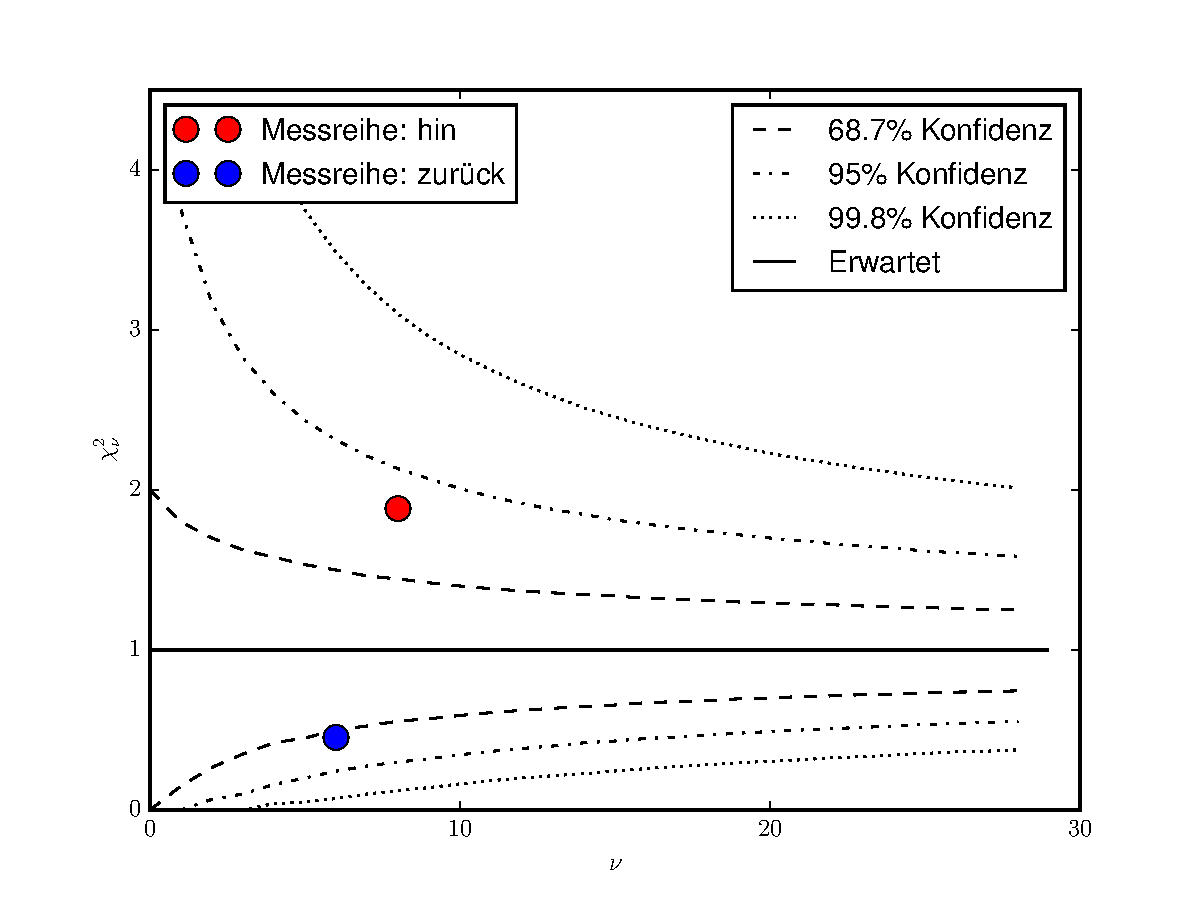
\includegraphics[width=450pt]{fotos/gpr1/M5_Chi_Quadrat.pdf}
		\caption[reduzierte Chi Quadrate]{reduzierte $  \chi^{2} $e von der Kalibrierung der Feder. \\Reduziertes $  \chi^{2} $ in Abhängigkeit der Freiheitsgrade $ \nu $}
		\label{Abb: Chi Quadrate}
	\end{figure}

Im folgenden habe ich für die Nachbesprechung die Abbildung (\ref{Abb: Hinweg}) nochmal überarbeitet. Aus den linearen Regressionen habe ich die Federkonstanten bestimmt und mit deren Hilfe die Oberflächenspannungen bestimmt. Beide Werte habe ich jeweils in eine Tabelle unter die jeweilige Grafik angegeben. Das Endergebnis habe ich jedoch nicht weiter verbessert.

\newpage

\begin{figure}[ht!]
	\centering
	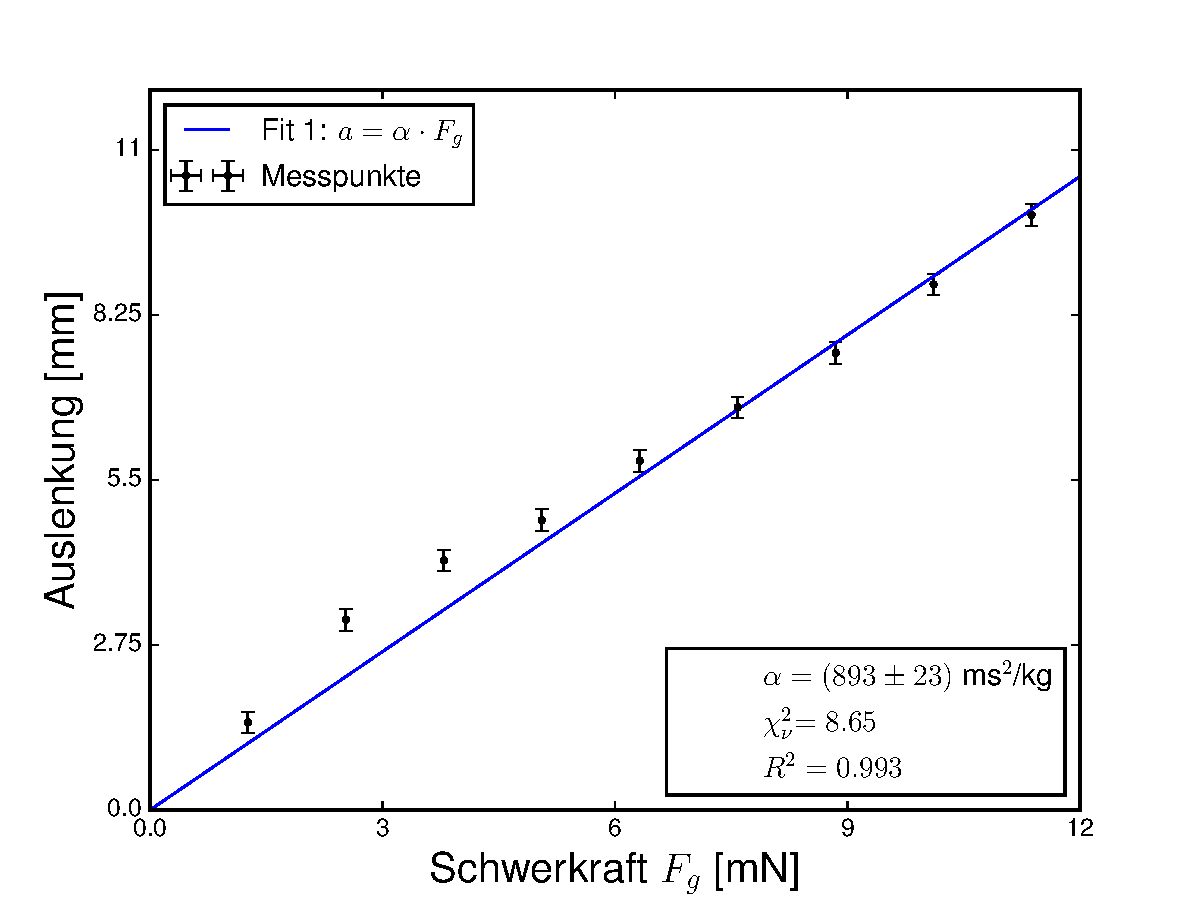
\includegraphics[width=400pt]{fotos/gpr1/M5_Hinweg_1.pdf}
	\caption[Regression 1 Korrektur 1]{lineare Regression zwischen Auslenkung $ a $ und der Gewichtskraft $ F_{g} $. Messpunkte sind an den einzelnen Kerben von 1 bis 9 (Hinweg, Zählung von 1, 2,..,9) in Abbildung gemacht worden. }
	\label{Abb: Hinweg1}
\end{figure}
\begin{table}[ht!]
	\centering
	\caption{Ergebnisse}
	\begin{tabular}{|c|c|}
		\hline
		& Platz 4 \\
		\hline
		Federkonstante [kg s$ ^{-2} $]& $k_{2}= 1.120\pm0.028 $ \\
		\hline
		Oberflächenspannung [mN$ \cdot $m$ ^{-1} $ ]& $\sigma_{2}= 58\pm 5$ \\
		\hline
	\end{tabular}
	\label{tab: Erg 2}
\end{table}


\newpage
\begin{figure}[ht!]
	\centering
	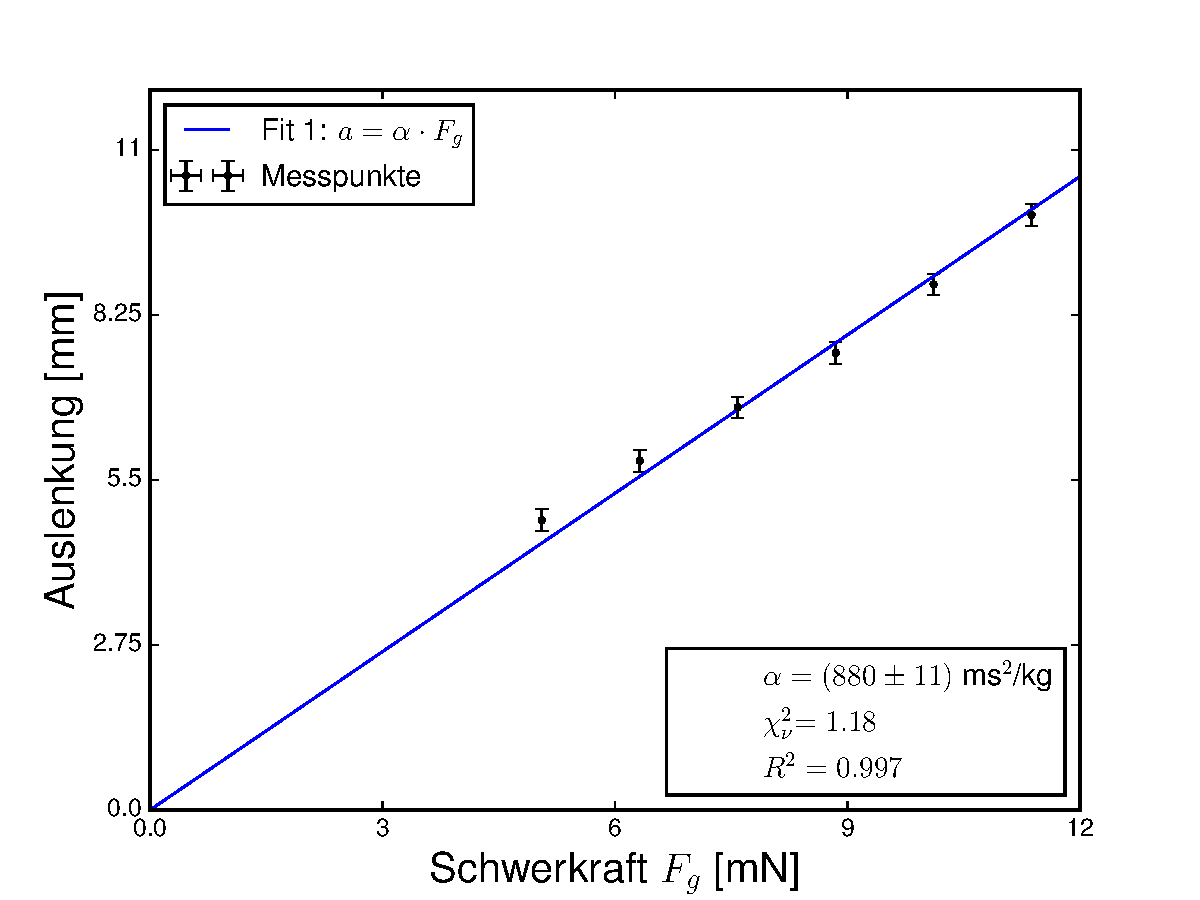
\includegraphics[width=400pt]{fotos/gpr1/M5_Hinweg_2.pdf}
	\caption[Regression 1 Korrektur 2]{lineare Regression zwischen Auslenkung $ a $ und der Gewichtskraft $ F_{g} $. Messpunkte sind an den einzelnen Kerben von 1 bis 9 (Hinweg, Zählung von 1, 2,..,9) in Abbildung gemacht worden. }
	\label{Abb: Hinweg2}
\end{figure}
\begin{table}[ht!]
	\centering
	\caption{Ergebnisse}
	\begin{tabular}{|c|c|}
		\hline
		& Platz 4 \\
		\hline
		Federkonstante [kg s$ ^{-2} $]& $k_{3}=1.136\pm 0.014  $ \\
		\hline
		Oberflächenspannung [mN$ \cdot $m$ ^{-1} $ ]& $\sigma_{3}= 59\pm 5 $ \\
		\hline
	\end{tabular}
	\label{tab: Erg 3}
\end{table}
